\section{The Squeeze Theorem And Some Special Limits}\label{sec:TrigLimits}


The previous section could have been titled ``Using Known Limits to Find Unknown Limits.'' By knowing certain limits of functions, we can find limits involving sums, products, powers, etc., of these functions. We further the development of such comparative tools with the Squeeze Theorem, a clever and intuitive way to find the value of some limits. 

In this section we aim to compute the limit:
$$\lim_{x\to0} {\sin x\over x}.$$

We start by analyzing the graph of $\ds{y=\frac{\sin x}{x}}$:
$$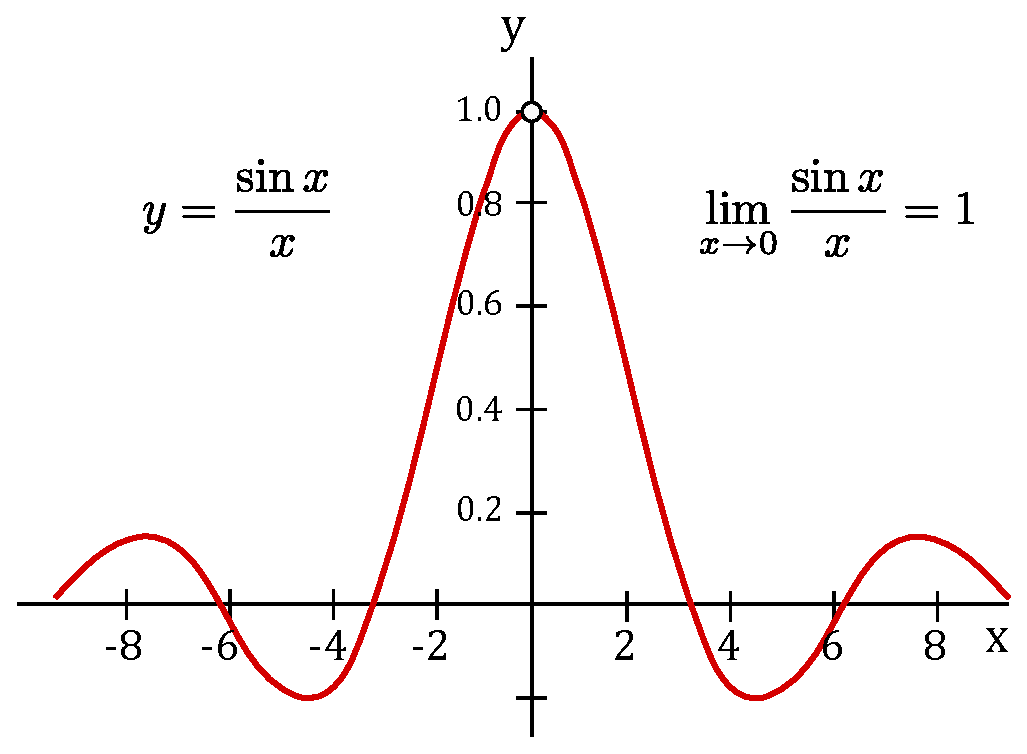
\includegraphics[width=3.0in]{images/sinx-over-x}$$
Notice that $x=0$ is not in the domain of this function.
Nevertheless, we can look at the limit as $x$ approaches $0$.
From the graph we find that the limit is $1$ (there is an open circle at $x=0$ indicating $0$ is not in the domain).
%We can expand upon the above limit and write it as follows:
%$$\lim_{x\to 0}\frac{\sin nx}{nx}=1.$$
We just convinced you this limit formula holds true based on the graph,
but how does one attempt to prove this limit more formally?
To do this we employ some indirect reasoning embodied in the \dfont{Squeeze Theorem}.

Before stating this theorem formally, suppose we have functions $f$, $g$ and $h$ where $g$ always takes on values between $f$ and $h$; that is, for all $x$ in an interval, $$f(x) \leq g(x) \leq h(x).$$ If $f$ and $h$ have the same limit at $c$, and $g$  is always ``squeezed'' between them, then $g$ must have the same limit as well. That is what the Squeeze Theorem states.

\begin{theorem}{Squeeze Theorem}{sqz}
{Let $f$, $g$ and $h$ be functions on an open interval $I$ containing $a$ such that for all $x$ in $I$, $$f(x)\leq g(x) \leq h(x).$$ If $$\lim_{x\to a} f(x) = L = \lim_{x\to a} h(x),$$ then $$\lim_{x\to a} g(x) = L.$$ \index{limit!Squeeze Theorem}\index{Squeeze Theorem}
}
\end{theorem}


\begin{center}
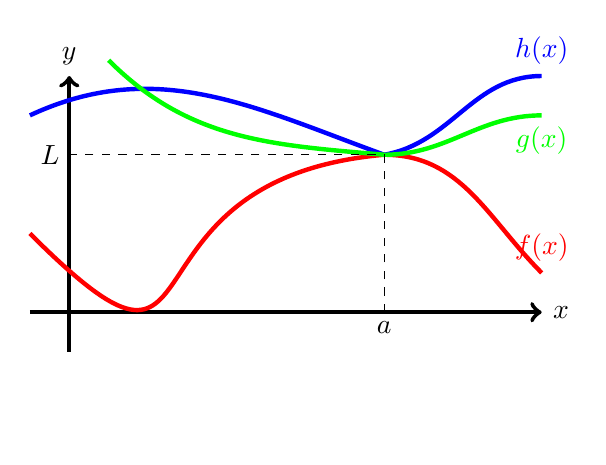
\begin{tikzpicture} %[default]
      %\diagram{-.5}{6}{-.5}{3}{1}
      \draw[->,ultra thick] (-.5,0)--(6,0) node[right]{$x$};
      \draw[->,ultra thick] (0,-.5)--(0,3) node[above]{$y$};
     % \diagramannotatez
      \draw[red,ultra thick] (-.5,1) to[out=-45,in=185,looseness=2] (4,2) to[out=0,in=135,looseness=1] node [at end,above] {$f(x)$} (6,.5);
      \draw[blue,ultra thick] (-.5,2.5) to[out=25,in=160,looseness=1] (4,2) to[out=10,in=180,looseness=1] node [at end,above] {$h(x)$} (6,3);
      \draw[green,ultra thick] (0.5,3.2) to[out=-45,in=175,looseness=1] (4,2) to[out=0,in=180,looseness=1] node [at end,below] {$g(x)$} (6,2.5);
      \draw[dashed] (4,0) -- node[at start,below] {$a$} (4,2) -- node[at end,left] {$L$} (0,2);
    \end{tikzpicture}
\end{center}

It can take some work to figure out appropriate functions by which to ``squeeze'' the given function of which you are trying to evaluate a limit. However, that is generally the only place work is necessary; the theorem makes the ``evaluating the limit part'' very simple. 

We use the Squeeze Theorem in the following example to finally prove that $\ds \lim_{x\to 0} \frac{\sin x}{x} = 1$.\\

\begin{example}{Using the Squeeze Theorem}{ex_limit_sinx_prove}{
Use the Squeeze Theorem to show that $$\ds \lim_{x\to 0} \frac{\sin x}{x} = 1.$$}
\end{example}


\begin{solution}
{We begin by considering the unit circle. Each point on the unit circle has coordinates $(\cos \theta,\sin \theta)$ for some angle $\theta$ as shown in Figure \ref{fig:squeeze_sinx}. Using similar triangles, we can extend the line from the origin through the point to the point $(1,\tan \theta)$, as shown. (Here we are assuming that $0\leq \theta \leq \pi/2$. Later we will show that we can also consider $\theta \leq 0$.)

\mfigure{.7}{The unit circle and related triangles.}{fig:squeeze_sinx}{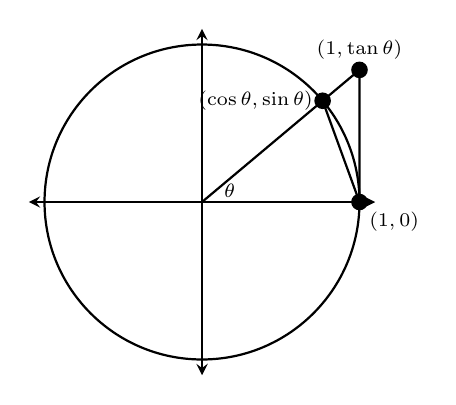
\begin{tikzpicture}[
>=stealth, scale=2]
\draw [thick] (0,0) node [shift={(10pt,4pt)}] {\scriptsize$\theta$} circle (1);
\draw [<->,thick] (-1.1,0) -- (1.1,0);
\draw [<->,thick] (0,-1.1) -- (0,1.1);
\draw [thick] (0,0) -- (1,.839) node [above] {\scriptsize$(1,\tan \theta)$}-- (1,0) -- (.766,.643);
\fill [black] (1,.839) circle (1.5pt);
\fill [black] (.766,.643) node [left] {\scriptsize$(\cos \theta,\sin \theta)$} circle (1.5pt);
\fill [black] (1,0) node [below right] {\scriptsize$(1,0)$} circle (1.5pt);
\end{tikzpicture}
}

Figure \ref{fig:squeeze_sinx} shows three regions have been constructed in the first quadrant, two triangles and a sector of a circle, which are also drawn below. The area of the large triangle is $\frac12\tan\theta$; the area of the sector is $\theta/2$; the area of the triangle contained inside the sector is $\frac12\sin\theta$. It is then clear from the diagram that we get the inequality in Figure \ref{fig:STpic}. 




\begin{figure}[H]
	\centering
	\begin{subfigure}[t]{0.33\textwidth}
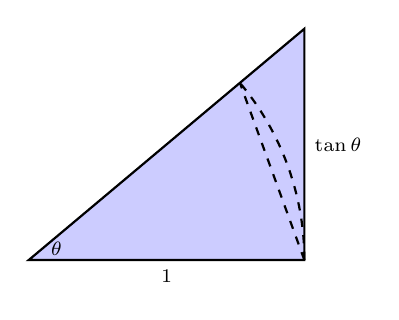
\begin{tikzpicture}[>=stealth,scale=3.5]
\fill [draw=black,thick,fill=blue!20] (0,0) node [shift={(10pt,4pt)}] {\scriptsize$\theta$} -- (1,.839) -- node [pos=.5,right] {\scriptsize$\tan \theta$} (1,0) -- cycle;
\draw (.5,0) node [below] {\scriptsize$1$};
\draw [black,dashed,thick] (1,0) arc (0:40:1);
\draw [black,dashed,thick] (1,0) -- (.766,.643);
\end{tikzpicture}		 
        \label{fig:STpica}
        \caption{$\ds \frac{\tan \theta}{2}$} 
    \end{subfigure}% 
    \begin{subfigure}[t]{0.33\textwidth}
     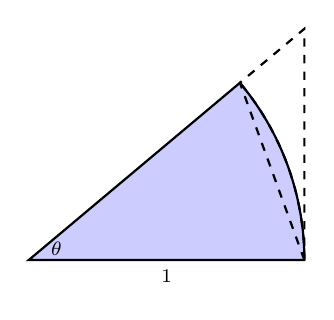
\begin{tikzpicture}[ %x=.5\marginparwidth,y=.5\marginparwidth,
     >=stealth,scale=3.5]
     \fill [draw=black,thick,fill=blue!20] (0,0) node [shift={(10pt,4pt)}] {\scriptsize$\theta$} -- (1,0) arc(0:40:1) -- cycle;
     \draw (.5,0) node [below] {\scriptsize$1$};
     \draw [black,dashed,thick] (1,0) arc (0:40:1);
     \draw [black,dashed,thick] (1,0) -- (.766,.643) -- (1,.839) -- cycle;
     \end{tikzpicture}
        \label{fig:STpicb}
        \caption{$\ds \frac{\theta}{2}$}    
    \end{subfigure}
\begin{subfigure}[t]{0.33\textwidth}
     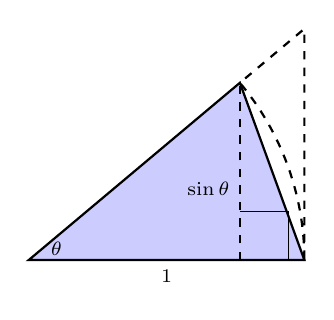
\begin{tikzpicture}[ %x=.5\marginparwidth,y=.5\marginparwidth,
     >=stealth,scale=3.5]
     \fill [draw=black,thick,fill=blue!20] (0,0) node [shift={(10pt,4pt)}] {\scriptsize$\theta$} -- (1,0) --(.766,.643) -- cycle;
     \draw [dashed,thick] (.766,0)  -- node [pos=.4,left] {\scriptsize$\sin \theta$}(.766,.643);
     \draw (.766,5pt) -- ++(5pt,0) -- ++(0,-5pt);
     \draw (.5,0) node [below] {\scriptsize$1$};
     %\draw [black,dashed] (1,0) arc (0:40:1);
     \draw [black,dashed,thick] (1,0) arc(0:40:1) --  (1,.839) -- cycle;
     \end{tikzpicture}
        \label{fig:STpicc}
        \caption{$\ds \frac{\sin \theta}{2}$}    
    \end{subfigure} 
    \caption{Demonstrating that $\ds \frac{\tan \theta}{2}  \geq \frac{\theta}{2} \geq \frac{\sin \theta}{2}$   \label{fig:STpic} }
\end{figure}


%\begin{center}
%\begin{tabular}{ccccc}
%\myincludegraphics{figures/figSqueeze1a} & & \myincludegraphics{figures/figSqueeze1b} & & \myincludegraphics{figures/figSqueeze1c}\\
%$\ds \frac{\tan \theta}{2}$\rule{0pt}{25pt} & $\geq$ & $\ds \frac{\theta}{2}$ & $\geq$ & $\ds \frac{\sin \theta}{2}$
%\end{tabular}
%\end{center}

%$$\frac{\tan\theta}{2} \geq \frac{\theta}{2} \geq \frac{\sin \theta}{2}.$$

Multiply all terms by $\ds\frac{2}{\sin \theta}$, giving $$\frac{1}{\cos\theta} \geq \frac{\theta}{\sin \theta} \geq 1.$$

Taking reciprocals reverses the inequalities, giving $$ \cos \theta \leq \frac{\sin \theta}{\theta} \leq 1.$$ (These inequalities hold for all values of $\theta$ near 0, even negative values, since $\cos (-\theta) = \cos \theta$ and $\sin (-\theta) = -\sin \theta$.)

Now take limits.

$$\lim_{\theta\to 0} \cos \theta \leq \lim_{\theta\to 0} \frac{\sin\theta}{\theta} \leq \lim_{\theta\to 0}  1 $$
$$\cos 0 \leq \lim_{\theta\to 0} \frac{\sin\theta}{\theta} \leq  1 $$
$$1 \leq \lim_{\theta\to 0} \frac{\sin\theta}{\theta} \leq  1 $$

Clearly this means that $\ds \lim_{\theta\to 0} \frac{\sin\theta}{\theta}=1$.\\
}
\end{solution}





Two notes about the previous example are worth mentioning. First, one might be discouraged by this application, thinking ``I would \textit{never} have come up with that on my own. This is too hard!'' Don't be discouraged; within this text we will guide you in your use of the Squeeze Theorem. As one gains mathematical maturity, clever proofs like this are easier and easier to create.


Second, this limit tells us more than just that as $x$ approaches $ 0 $, $\sin(x)/x$ approaches $ 1 $. Both $x$ and $\sin x$ are approaching $ 0 $, but the \textit{ratio} of $x$ and $\sin x$ approaches $ 1 $, meaning that they are approaching $ 0 $ in essentially the same way. Another way of viewing this is: for small $x$, the functions $y=x$ and $y=\sin x$ are essentially indistinguishable.\\


We include this special limit, along with three others, in the following theorem.

\begin{theorem}{Special Limits}{special_limits}{%
\noindent\begin{minipage}[t]{.5\textwidth}
\begin{enumerate}
	\item		$\ds \lim_{x\to 0} \frac{\sin x}{x} = 1$
	\item		$\ds \lim_{x\to 0} \frac{\cos x-1}{x} = 0$
\end{enumerate}
\end{minipage}
\begin{minipage}[t]{.5\textwidth}
\begin{enumerate}\addtocounter{enumi}{2}
	\item		$\ds \lim_{x\to 0} (1+x)^\frac1x = e$
	\item		$\ds \lim_{x\to 0} \frac{e^x-1}{x} = 1$
\end{enumerate}
\end{minipage}
}
\end{theorem}


A short word on how to interpret the latter three limits. We know that as $x$ goes to 0, $\cos x$ goes to 1. So, in the second limit, both the numerator and denominator are approaching 0. However, since the limit is 0, we can interpret this as saying that ``$\cos x$ is approaching 1 faster than $x$ is approaching 0.''

In the third limit, inside the parentheses we have an expression that is approaching 1 (though never equaling 1), and we know that 1 raised to any power is still 1. At the same time, the power is growing toward infinity. What happens to a number near 1 raised to a very large power? In this particular case, the result approaches Euler's number, $e$, approximately $2.718.$

In the fourth limit, we see that as $x\to 0$, $e^x$ approaches 1 ``just as fast'' as $x\to 0$, resulting in a limit of 1.\\


\begin{example}{Limit of Other Trig Functions}{LimitOtherTrigFunctions}
Compute the following limit $\ds\lim_{x\to 0}\frac{\sin 5x\cos x}{x}$.
\end{example}

\begin{solution} 
We have
$$\begin{array}{rcl}
\ds{\lim_{x\to 0}\frac{\sin 5x\cos x}{x}} & = & \ds{\lim_{x\to 0}\frac{5\sin 5x\cos x}{5x}}\\
\\
~ & = & \ds{\lim_{x\to 0} 5\cos x\left(\frac{\sin 5x}{5x}\right)}\\
\\
~ & = &  5\cdot (1)\cdot (1)~~=~~5\\
\end{array}$$
since $\cos(0)=1$ and $\ds{\lim_{x\to 0}\frac{\sin 5x}{5x}=1}$.
\end{solution}
Let's do a harder one now.

\begin{example}{Limit of Other Trig Functions}{LimitOtherTrigFunctions2}
Compute the following limit:
$\ds\lim_{x\to 0}\frac{\tan^3 2x}{x^2\sin 7x}$.
\end{example}

\begin{solution} 
Recall that the $\tan^3(2x)$ means that $\tan(2x)$ is being raised to the third power.
$$\begin{array}{rcll}
\ds{\lim_{x\to 0}\frac{\tan^3(2x)}{x^2\sin(7x)}}&=& \ds{\lim_{x\to 0}\frac{(\sin(2x))^3}{x^2\sin(7x)\cos^3(2x)}}
& \mbox{Rewrite in terms of $\sin$ and $\cos$}\\
\\
~&=&\ds{\lim_{x\to 0}\frac{(2x)^3\left(\frac{\sin(2x)}{2x}\right)^3}{x^2(7x)\left(\frac{\sin(7x)}{7x}\right)\cos^3(2x)}}
& \mbox{Make sine terms look like: $\ds{\frac{\sin\theta}{\theta}}$}\\
\\
~&=&\ds{\lim_{x\to 0}\frac{8x^3(1)^3}{7x^3(1)(1^3)}} 
& \mbox{Replace $\ds{\lim_{x\to 0}\frac{\sin nx}{nx}}$ with $1$. Also, $\cos(0)=1$.}\\
\\
~&=&\ds{\lim_{x\to 0}\frac{8}{7}}&\mbox{Cancel $x^3$'s.}\\
\\
~&=&\ds{\frac{8}{7}}.\\
\end{array}$$
\end{solution}

\begin{example}{Applying the Squeeze Theorem}{Applying the Squeeze Theorem}
Compute the following limit:
$\ds\lim_{x\to 0^+}x^3\cos\left(\frac{1}{\sqrt{x}}\right)$.
\end{example}

\begin{solution} 
We use the \ifont{Squeeze Theorem} to evaluate this limit.
We know that $\cos\alpha$ satisfies $-1\leq\cos\alpha\leq 1$ for any choice of $\alpha$.
Therefore we can write:
$$-1\leq\cos\left(\frac{1}{\sqrt{x}}\right)\leq 1$$
Since $x\to 0^+$ implies $x>0$, multiplying by $x^3$ gives:
$$-x^3\leq x^3\cos\left(\frac{1}{\sqrt{x}}\right)\leq x^3.$$
$$\lim_{x\to 0^+}(-x^3)\leq \lim_{x\to 0^+}\left(x^3\cos\left(\frac{1}{\sqrt{x}}\right)\right)\leq\lim_{x\to 0^+} x^3.$$
But using our rules we know that
$$\lim_{x\to 0^+}(-x^3)=0,\qquad\qquad \lim_{x\to 0^+} x^3=0$$
and the Squeeze Theorem says that the only way this can happen is if
$$\lim_{x\to 0^+}x^3\cos\left(\frac{1}{\sqrt{x}}\right)=0.$$
\end{solution}


%\begin{theorem}{Squeeze Theorem}{SqueezeTheorem}
%Suppose that $g(x) \le f(x) \le h(x)$ for all $x$ close to $a$ but not
%equal to $a$. If $\ds\lim_{x\to a}g(x)=L=\lim_{x
%\to a}h(x)$, then $\ds\lim_{x\to a}f(x)=L$.
%\end{theorem}
% 
%This theorem can be proved using the official definition of limit. We
%won't prove it here, but point out that it is easy to understand and
%believe graphically. The condition says that $f(x)$ is trapped between
%$g(x)$ below and $h(x)$ above, and that at $x=a$, both $g$ and $h$
%approach the same value. This means the situation looks something like
%Figure~\ref{fig:squeeze}.
%
%For example, imagine the blue curve is $f(x)=x^2\sin(\pi/x)$, the
%upper (red) and lower (green) curves are $h(x)=x^2$ and $g(x)=-x^2$. Since the sine function
%is always between $-1$ and $1$, $-x^2\le x^2\sin(\pi/x)\le x^2$, and
%it is easy to see that $\lim_{x\to0}-x^2=0=\lim_{x\to0}x^2$.
%It is not so easy to see directly (i.e. algebraically) that 
%$\lim_{x\to0}x^2\sin(\pi/x)=0$, because the $\pi/x$ prevents us from
%simply plugging in $x=0$. The squeeze theorem makes this ``hard
%limit'' as easy as the trivial limits involving $x^2$.

%\figure[!ht]
%\centerline{\vbox{\beginpicture
%\normalgraphs
%%\ninepoint
%\setcoordinatesystem units <4truecm,4truecm>
%\setplotarea x from -1 to 1, y from -1 to 1
%\axis left shiftedto x=0 /
%\axis bottom shiftedto y=0 /
%\setquadratic
%\plot -1.000 0.000 -0.980 0.060 -0.961 0.118 -0.941 0.173 -0.922 0.224
%-0.902 0.272 -0.882 0.317 -0.863 0.357 -0.843 0.392 -0.824 0.423
%-0.804 0.448 -0.784 0.468 -0.765 0.481 -0.745 0.488 -0.726 0.488
%-0.706 0.481 -0.686 0.467 -0.667 0.445 -0.647 0.415 -0.628 0.377
%-0.608 0.332 -0.588 0.280 -0.569 0.223 -0.549 0.161 -0.530 0.096
%-0.510 0.032 -0.490 -0.030 -0.471 -0.084 -0.451 -0.128 -0.432 -0.156
%-0.412 -0.165 -0.392 -0.152 -0.373 -0.117 -0.353 -0.063 -0.334 -0.001
%-0.314 0.054 -0.294 0.082 -0.275 0.068 -0.255 0.016 -0.236 -0.039
%-0.216 -0.043 -0.196 0.011 -0.177 0.028 -0.157 -0.022 -0.138 0.014
%-0.118 -0.014 -0.098 -0.005 -0.079 -0.005 -0.059 -0.001 -0.040 0.001
%-0.020 0.000 0 0
%0.020 0.000 0.040 -0.001 0.059 0.001 0.079 0.005 0.098 0.005
%0.118 0.014 0.138 -0.014 0.157 0.022 0.177 -0.028 0.196 -0.011
%0.216 0.043 0.236 0.039 0.255 -0.016 0.275 -0.068 0.294 -0.082
%0.314 -0.054 0.334 0.001 0.353 0.063 0.373 0.117 0.392 0.152
%0.412 0.165 0.432 0.156 0.451 0.128 0.471 0.084 0.490 0.030
%0.510 -0.032 0.530 -0.096 0.549 -0.161 0.569 -0.223 0.588 -0.280
%0.608 -0.332 0.628 -0.377 0.647 -0.415 0.667 -0.445 0.686 -0.467
%0.706 -0.481 0.726 -0.488 0.745 -0.488 0.765 -0.481 0.784 -0.468
%0.804 -0.448 0.824 -0.423 0.843 -0.392 0.863 -0.357 0.882 -0.317
%0.902 -0.272 0.922 -0.224 0.941 -0.173 0.961 -0.118 0.980 -0.060
%1.000 0.000 /
%\plot -1 1 0 0 1 1 /
%\plot -1 -1 0 0 1 -1 /
%\endpicture}}
%\caption{The squeeze theorem. \label{fig:squeeze}}
%\endfigure

%\begin{figure}[!ht]
%$$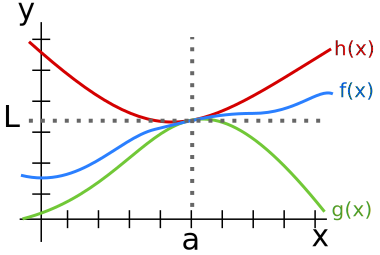
\includegraphics[width=3.0in]{images2/squeeze-theorem}$$
%\caption{The squeeze theorem. \label{fig:squeeze}}
%\end{figure}
%
%To compute $\ds\lim_{x\to0}
%(\sin x)/x$, we will find two simpler functions $g$ and $h$ so that 
%$g(x)\le (\sin x)/x\le h(x)$, and so that
%$\lim_{x\to0}g(x)=\lim_{x\to0}h(x)$. Not too surprisingly, this will
%require some trigonometry and geometry. Referring to
%figure~\ref{fig:hard limit}, $x$ is the measure of the angle in
%radians. Since the circle has radius 1, the coordinates of point $A$
%are $(\cos x,\sin x)$, and the area of the small triangle is 
%$(\cos x\sin x)/2$. This triangle is completely contained within the
%circular wedge-shaped region bordered by two lines and the circle from
%$(1,0)$ to point $A$. Comparing the areas of the triangle and the
%wedge we see
%$(\cos x\sin x)/2 \le x/2$, since the area of a circular region with
%angle $\theta$ and radius $r$ is $\theta r^2/2$. With a little algebra
%this turns into $(\sin x)/x \le 1/\cos x$, giving us the $h$ we seek.
%
%\figure[!ht]
%\centerline{\vbox{\beginpicture
%\normalgraphs
%%\ninepoint
%\setcoordinatesystem units <4truecm,4truecm>
%\setplotarea x from 0 to 1, y from 0 to 1
%\circulararc 90 degrees from 1 0 center at 0 0
%\axis left ticks numbered from 0 to 1 by 1 /
%\axis bottom ticks numbered from 1 to 1 by 1 /
%\putrule from  0.8660254040 0 to 0.8660254040 0.5
%\putrule from  1 0 to 1 .577
%\plot 0 0 1 .577 /
%\put {$x$} [bl] <5pt,2.5pt> at 0.1 0
%\put {$A$} [r] <-6pt,2pt> at 0.8660254040 0.5
%\put {$B$} [bl] <3pt,3pt> at 1  .577
%\circulararc 30 degrees from 0.1 0 center at 0 0
%\endpicture}}
%\caption{Visualizing $\sin x / x$. \label{fig:hard limit}}
%\endfigure
%
%To find $g$, we note that the circular wedge is completely contained
%inside the larger triangle. The height of the triangle, from $(1,0)$
%to point $B$, is $\tan x$, so comparing areas we get
%$x/2 \le (\tan x)/2 = \sin x / (2\cos x)$. With a little algebra this
%becomes $\cos x \le (\sin x)/x$. So now we have 
%$$ \cos x \le {\sin x\over x}\le {1\over\cos x}.$$
%Finally, the two limits $\lim_{x\to0}\cos x$ and $\lim_{x\to0}1/\cos x$
%are easy, because $\cos(0)=1$. By the squeeze theorem,
%$\lim_{x\to0} (\sin x)/x = 1$ as well.
%
%Using the above, we can compute a similar limit:
%$$\lim_{x\to0}{\cos x - 1\over x}.$$
%This limit is just as hard as $\sin x/x$, but closely related to it,
%so that we don't have to do a similar calculation; instead we can do a
%bit of tricky algebra.
%$${\cos x - 1\over x}={\cos x - 1\over x}{\cos x+1\over\cos x+1}
%={\cos^2 x - 1\over x(\cos x+1)}={-\sin^2 x\over x(\cos x+1)}=
%-{\sin x\over x}{\sin x\over \cos x + 1}.$$
%To compute the desired limit it is sufficient to compute the limits of
%the two final fractions, as $x$ goes to 0. The first of these is the
%hard limit we've just done, namely 1. The second turns out to be
%simple, because the denominator presents no problem:
%$$\lim_{x\to0}{\sin x\over \cos x + 1}={\sin 0\over \cos 0+1}=
%{0\over 2}  = 0.$$
%Thus,
%$$\lim_{x\to0}{\cos x - 1\over x}=0.$$



When solving problems using the Squeeze Theorem it is also helpful to have the following theorem.

\begin{theorem}{Monotone Limits}{MonotoneLimits}\label{MonotoneLimits} 
If $f(x)\leq g(x)$ when $x$ is near $a$ (except possibly at $a$) and the limits of $f$ and $g$ both exist as $x$ approaches $a$, then $\ds\lim_{x\to a}f(x)\leq\lim_{x\to a}g(x)$.
\end{theorem}


%%%%%%%%%%%%%%%%%%%%%%%%%%%%%%%%%%%%%%%%%
\Opensolutionfile{solutions}[ex]
\section*{Exercises for \ref{sec:TrigLimits}}

\begin{enumialphparenastyle}

%%%%%%%%%%
\begin{ex}
Compute the following limits.
\begin{enumerate}
	\item	$\ds\lim_{x\to 0} {\sin (5x)\over x}$
	\item	$\ds\lim_{x\to 0 } {\sin(7x)\over\sin (2x)}$
	\item	$\ds\lim_{x\to 0 } {\cot (4x) \over\csc (3x)}$
	\item	$\ds\lim_{x\to 0 } {\tan x\over x}$
	\item	$\ds\lim_{x\to \pi/4} {\sin x-\cos x \over\cos (2x)}$
\end{enumerate}
\begin{sol}
\begin{enumerate}
	\item	$5$
	\item	$7/2$
	\item	$3/4$
	\item	$1$
	\item	$-\sqrt2/2$
\end{enumerate}
\end{sol}
\end{ex}

%%%%%%%%%%
\begin{ex} 
For all $x\geq 0$, $4x-9 \leq f(x) \leq x^2 - 4x +7$. Find $\ds\lim_{x\to4}f(x)$.
\begin{sol}
 $7$
\end{sol}
\end{ex}

%%%%%%%%%%
\begin{ex} 
For all $x$, $2x \leq g(x) \leq x^4 - x^2 +2$. Find $\ds\lim_{x\to1}g(x)$.
\begin{sol}
 $2$
\end{sol}
\end{ex}

% % % % % % % % % % %
\begin{ex}
{Use the Squeeze Theorem where appropriate, to evaluate the given limit.}

\begin{enumerate}
\item {$\ds \lim_{x\to0} x\sin\left(\frac{1}{x}\right)$}

\item {$\ds \lim_{x\to0} \sin x\cos\left(\frac{1}{x^2}\right)$}

\item {$\ds \lim_{x\to0} x\sin\left(\frac{1}{x}\right)$}

\item {$\ds \lim_{x\to3^+} f(x)$, where $6x-9\leq f(x) \leq x^2$ on $[0,3]$.}

\end{enumerate}

\begin{sol}
\begin{enumerate}
\item {$0$}
\item {$0$}
\item {$0$}
\item {$9$}
\end{enumerate}
\end{sol}

\end{ex}
% % % % % % % % % % % %





%%%%%%%%%%
\begin{ex} 
Use the Squeeze Theorem to show that $\ds\lim_{x\to0} x^4 \cos(2/x)=0$.
\end{ex}


%%%%%%%%%%
\begin{ex}
Find the value of $\lim_{x\to\infty}\dfrac{3x+\sin x}{x+\cos x}$. Justify your steps carefully.
\begin{sol}
	$ 3 $
\end{sol}
\end{ex}


% % % % % % % % % % %
\begin{ex}
{\noindent The following exercises}
{ challenge your understanding of limits but can be evaluated using the knowledge gained in this section.}
\begin{enumerate}
\item {$\ds \lim_{x\to0}\frac{\sin 3x}{x}$}

\item {$\ds \lim_{x\to0}\frac{\sin 5x}{8x}$}

\item {$\ds \lim_{x\to0}\frac{\ln (1+x)}{x}$}

\item {$\ds \lim_{x\to0}\frac{\sin x}{x}$, where $x$ is measured in degrees, not radians.}

\end{enumerate}

\begin{sol}
\begin{enumerate}
\item {$3$}
\item {$5/8$}
\item {$1$}
\item {$\pi/180$}
\end{enumerate}
\end{sol}

\end{ex}
% % % % % % % % % % % %


\end{enumialphparenastyle}
